\capitulo{3}{Conceptos teóricos}

\section{Conceptos teóricos básicos}

\subsection{Enfermedad de Párkinson}
La enfermedad de Párkinson es un trastorno neurodegenerativo del sistema nervioso central caracterizado por la pérdida de neuronas dopaminérgicas en los ganglios basales (sustancia negra), derivando en una deficiencia de dopamina que afecta a la regulación de las estructuras cerebrales implicadas en el control del movimiento. \\ \\
Se trata del trastorno neurodegenerativo muscular más común, con unos ratios de incidencia de 11–19/100 000 casos y de prevalencia de 108–257/100 000 casos al año en Europa. \cite{balestrino2020parkinson}

\subsubsection{Causas}
Las causas de la enfermedad de Párkinson no han sido claramente establecidas. Sin embargo, hay un creciente consenso sobre la convergencia de ciertos mecanismos autónomos celulares y mecanismos no autónomos celulares como causas del deterioro de las neuronas dopaminérgicas\cite{hirsch2013pathogenesis}:
\begin{itemize}
    \item Mecanismos autónomos celulares: La regulación por el coactivador transcripcional PGC-1 alfa se encuentra alterada en pacientes con gen parkin no funcional. Esta regulación es esencial para la biogénesis mitocondrial, el metabolismo de especies reactivas del oxígeno (ROS) y la respiración celular.\\
    La sobreexpresión de proteína PARIS causada por la inactivación del gen parkin  reprime la expresión del coactivador transcripcional PGC-1 alfa, impidiendo la activación de NRF-1 (factor respiratorio nuclear 1), el cual es clave en la respiración mitocondrial. \cite{SHIN2011689}
    \item Mecanismos no autónomos celulares: La agregación anormal de proteínas, en particular de la  alfa-sinucleína (alfa-syn) causa degeneración neuronal en la sustancia negra y en el cuerpo estriado. \\
    La alfa-syn es una proteína presente en los terminales presinápticos de las neuronas, la cual resulta esencial para el correcto funcionamiento mitocondrial.  La acumulación de oligómeros y agregados más grandes de alfa-syn mal plegada, debido a factores genéticos o ambientales, se propaga en pacientes con párkinson a lo largo de las distintas etapas de la enfermedad mediante un mecanismo similar al de los priones, llegando a afectar numerosas áreas como el bulbo olfatorio, el cortex cerebral o la amígdala y produciendo diferente sintomatología en el paciente según las áreas afectadas. \cite{10.3389/fnins.2019.00552}
\end{itemize}
La acumulación de mitocondrias disfuncionales causada por una deficiente función de parkin y PINK1 (que eliminarían mitocondrias disfuncionales en condiciones normales) resulta en una pérdida de función de neuronas dopaminérgicas de la sustancia negra, derivando en una progresiva pérdida de funciones cerebrales. \cite{hirsch2013pathogenesis}
\subsubsection{Diagnóstico y sintomatología}
El primer paso hacia un diagnóstico de párkinson es la detección de parkinsonismo, basándose este término en 3 manifestaciones motoras cardinales, las cuales deben aparecer claramente y sin otra causa definida\cite{postuma2015mds}: 
\begin{itemize}
    \item Bradicinesia: ralentización de los movimientos y disminución de su amplitud. Debe estar presente combinada con al menos una de las siguientes manifestaciones.
    \item Temblores en reposo
    \item Rigidez
\end{itemize}
La Sociedad de Trastornos del movimiento (MDS) establece una guía para diagnosticar parkinson de forma clínica o una probabilidad de párkinson. Para ello describe 
una serie de criterios de exclusión, criterios de apoyo y banderas rojas.\cite{postuma2015mds}

\subsubsection{Tratamiento de los síntomas motores}
Existen numerosas formas de tratar los síntomas motores en pacientes con párkinson. La elección en el tratamiento farmacológico del paciente dependerá en gran medida de la edad y el compromiso funcional que presentan los pacientes. Algunos de los tratamientos farmacológicos utilizados para tratar la sintomatología motora son \cite{marin2018enfermedad}:
\begin{itemize}
    \item Levodopa: Fármaco precursor de la dopamina, el cual se transforma en esta sustancia tras la acción de la enzima dopa-descarboxilasa. Para asegurar el paso a través de la barrera hematoencefálica previo a esta reacción se utiliza conjuntamente con inhibidores de la enzima dopa-descaroxilasa periférica, como la carbidopa y la benserazida. \\
    Es el fármaco más utilizado para el tratamiento de los síntomas motores de la enfermedad de Párkinson, debido a su efectividad en la reducción de temblores, bradicinesia y rigidez. Sin embargo, la toma a largo plazo durante 5-10 años produce complicaciones en más de la mitad de los pacientes, por lo cual su administración suele intentar evitarse en los pacientes más jóvenes.
    \item Agonistas dopaminérgicos: Medicamentos que estimulan los receptores de dopamina, aumentando de esta forma los efectos de esta sustancia en los pacientes sin aumentar la concentración de la misma. Producen menos fluctuaciones motoras y discinesias en comparación con la levodopa. Sin embargo, su eficacia se reduce conforme avanza la enfermedad, siendo necesario en estas etapas el acompañamiento de fármacos como la levodopa para poder manejar los crecientes síntomas.
    \item Inhibidores de la monoaminooxidasa tipo B (iMAO-B): Medicamentos como la selegilina, rasagilina y safinamida inhiben la enzima MAO-B, encargada de descomponer la dopamina en el cerebro. De esta forma se consigue un aumento en los niveles y efecto de la dopamina, consiguiendo una leve mejoría de los síntomas. Esto los hace ideales candidatos para un tratamiento inicial.
    \item Amantadina: Este medicamento tiene múltiples efectos beneficiosos: Produce un aumento en la liberación de dopamina en neuronas presinápticas, evitando también su recaptación; bloquea los receptores NMDA, lo cual puede reducir las discinesias causadas por el consumo de levodopa y también presenta leves efectos anticolinérgicos.
    \item Anticolinérgicos: Sustancias que bloquean la acción de la acetilcolina en el sistema nervioso, pueden reducir el temblor y la rigidez muscular. Estos medicamentos se administran aumentando progresivamente las dosis para intentar evitar efectos adversos que resultan muy comunes. Resultan útiles en pacientes con temblores que no responden a levodopa o agonistas dopaminérgicos.
    \item Inhibidores de la Catecol-O-metiltransferasa (i-COMT): Estos medicamentos evitan el paso de L-dopa a 3-O-metildopa, aumentando con ello la vida media de la levodopa y reduciendo las fluctuaciones motoras causadas por este tratamiento al usarse junto con él.
    
\end{itemize}

\subsection{Diario de fluctuaciones motoras}

Los estados de respuesta al tratamiento en pacientes con Párkinson fluctuan de forma regular entre el estado \textit{ON}, descrito como un periodo de efectividad de las medicaciones durante el cual los síntomas motores se encuentran controlados, y el estado \textit{OFF}, en el cual descienden los efectos de las medicaciones y los síntomas empeoran, entorpeciendo la movilidad del paciente. Este último estado suele tener lugar en los instantes previos a una nueva toma de la medicación.

La detección de periodos \textit{ON} y \textit{OFF}, así como la distinción entre periodos \textit{ON} con o sin discinesia (movimientos involuntarios) por parte del paciente resulta esencial para la evaluación de la efectividad del tratamiento. Debido a ello, el diario de fluctuaciones creado por Hauser et al. en el año 2000 \cite{hauser2000home}, en el cual los pacientes determinan a lo largo del día si se encuentran en estado \textit{OFF} o en estado \textit{ON} (especificando en este caso en nivel de discinesia) ha sido ampliamente utilizado durante la realización de ensayos clínicos con el objetivo de probar la eficacia de diferentes medicaciones en la enfermedad de párkinson, así como por neurólogos para evaluar la eficacia del tratamiento prescrito.



\section{Estado del arte y trabajos relacionados.}
Con el objetivo de entender el estado actual en la industria de los recursos y proyectos de ayuda y monitorización de Párkinson, se presenta una revisión bibliográfica, incluyendo información sobre aquellos trabajos más relacionados con el presente proyecto.

\subsection{Revisión de recursos para la monitorización y ayuda de pacientes con Párkinson}

\subsubsection{Plataformas web en la monitorización de enfermedad de párkinson}
En el artículo 'Mobile phone applications in Parkinson's disease: a systematic review' \cite{LINARESDELREY201938} encontramos una revisión sistemática de las aplicaciones móviles utilizadas en la enfermedad de Párkinson. 33 de estas aplicaciones incluyen funciones de evaluación, monitorizando síntomas motores como la marcha, el equilibrio, los temblores, el habla... Entre ellas, se resumen las funciones de algunas de las más relevantes para el presente proyecto, diseñadas para monitorizar síntomas motores en la marcha:
\begin{itemize}
    \item 'A Mobile Kalman-Filter Based Solution for the Real-Time Estimation of Spatio-Temporal Gait Parameters' \cite{7173053} presenta una aplicación Android que permite a los usuarios monitorear su marcha y registrar datos relevantes para el análisis y monitoreo de la misma. Esta aplicación procesa datos obtenidos de un sistema PDR (Pedestrian Dead Reckoning), compuesto por dos IMUs situadas en los zapatos del usuario. La aplicación muestra parámetros relacionados con las características de la marcha en ambos pies, como se muestra en la figura \ref{fig:androidappmarcha}.
    \begin{figure}[h]
        \centering
        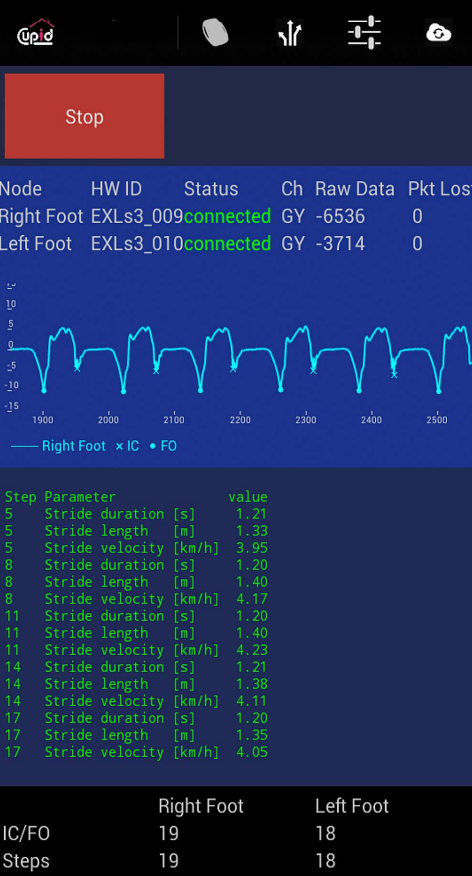
\includegraphics[width=0.5\textwidth]{img/Androidapp1.png}
        \caption{Captura de la apicación Android diseñada en \cite{7173053}}
        \label{fig:androidappmarcha}
    \end{figure}
    \item 'Unconstrained detection of freezing of Gait in Parkinson's disease patients using smartphone' \cite{7319209} propone una aplicación para dispositivos Android que permite recopilar los datos obtenidos con los sensores de acelerómetro y giroscopio presentes en el teléfono inteligente  Google Nexus 5  durante la marcha del paciente. Estos datos se procesan con el objetivo de clasificarlos entre episodios de congelación de la marcha y marcha normal. Esta aplicación tiene el propósito de detectar estos episodios, sin estar destinada al uso futuro de la misma por parte de un cliente.
    \item 'Feasibility and effects of home-based smartphone-delivered automated feedback training for gait in people with Parkinson's disease: A pilot randomized controlled trial' \cite{GINIS201628} presenta la aplicación CuPiD (Cueing and Prompting in Parkinson's Disease), diseñada para ayudar a los pacientes con Párkinson a controlar los episodios de congelación de la marcha y mejorar la calidad global de su marcha. Utiliza datos recogidos con sensores de movimiento sobre la marcha del paciente para proporcionar un feedback en tiempo real sobre la marcha del usuario y ofrecer instrucciones auditivas o visuales para mejorarla. Esta app demostró ser más eficaz en la mejora del equilibrio en pacientes con Párkinson que el entrenamiento de la marcha convencional.
\end{itemize}
\subsubsection{Análisis de la marcha en pacientes con enfermedades neurodegenerativas mediante dispositivos electrónicos portátiles}
El artículo 'Assessing Gait in Parkinson’s Disease Using Wearable Motion Sensors: A Systematic Review', escrito en 2019 por L. Brognara et al\cite{diseases7010018} se destaca la utilidad de las unidades de medición inercial (IMU), frecuentemente presentando funciones de acelerómetro y giroscopio, en el análisis objetivo de los movimientos en pacientes con enfermedades neurodegenerativas. Se destaca esta opción por la utilidad que presentan características como el reducido tamaño y coste de los mismos, que los hacen adecuados para el uso en contextos clínicos y fuera de ellos. En este texto se hace una revisión de artículos que posicionan los IMU en diferentes partes del cuerpo, siendo ambos tobillos la segunda localización más utilizada. \\

Este posicionamiento de sensores, así como la localización en la zona lumbar se utilizan en el artículo 'Wearables for gait and balance assessment in the neurological ward - study design and first results of a prospective cross-sectional feasibility study with 384 inpatients' \cite{Bernhard2018}, en el que se analiza el equilibrio y la marcha de pacientes neurológicos hospitalizados, la mayoría presentando patologías como Párkinson, ictus o leucemia. Se concluye la gran utilidad y fiabilidad de los dispositivos portables con acelerómetros 3D en la evaluación de estos parámetros en pacientes neurológicos.\\

\subsubsection{Líneas transversales en el suelo como ayuda visual al inicio de la marcha en pacientes con Párkinson}
El artículo 'Effects of visual and auditory cues on gait initiation in people with Parkinson's disease' \cite{doi:10.1191/0269215506cr925oa} describe la efectividad del uso de líneas transversales en la iniciación de la marcha de pacientes con Párkinson, destacando la mejora en la magnitud del inicio de la marcha: los pacientes que utilizan esta ayuda en el inicio de la marcha toman un primer paso con mayor fuerza, recorriendo una mayor longitud. Esto se mantiene a lo largo de la marcha, resultando en una velocidad promedio mayor.\\

Por otro lado, el artículo presentado por Chan et al.\cite{10.3389/fbioe.2024.1334403} investiga el efecto de la proyección de líneas láser como estímulo visual en pacientes con Párkinson. Se propone un dispositivo integrado en ambos zapatos del paciente, que utiliza la presión ejercida por el pie en la suela y la inercia para detectar el movimiento de cada pie, activando la proyección de línea láser en el pie contrario. De esta forma se proporciona en todo momento una ayuda visual al paciente durante la marcha. En pacientes con síntomas motores más agudos la ayuda de este dispositivo redujo la cantidad de episodios de congelación de la marcha.\\

El artículo presentado por Velik et al. \cite{6347005} describe que el uso de proyecciones de líneas láser paralelas en el suelo además de reducir significativamente la cantidad de episodios de congelación de la marcha, reduce su duración en un 51 por ciento con la proyección de líneas láser de forma continuada y un 69 por ciento con la proyección de líneas láser 'por demanda'.

\subsection{Proyectos relacionados}
\begin{itemize}
\item El artículo 'Gait monitoring system for patients with Parkinson’s disease' \cite{GONCALVES2021115653} presenta un sistema de monitorización de la marcha en pacientes con Párkinson, constituido por una unidad de medición inercial (IMU), con un sensor MPU-6050, el cual se utiliza para adquirir datos inerciales.\\

Este sensor se encuentra situado en un cinturón, que incluye también una unidad de almacenamiento de datos, una unidad de procesamiento con un algoritmo de detección de eventos de la marcha, el cual utiliza un microcontrolador Atmega 2560 y un módulo bluetooth. Este módulo se utiliza para comunicarse con una aplicación Android, que permite graficar los datos e iniciar/finalizar de forma inalámbrica el funcionamiento del dispositivo.
\item El artículo presentado por Takač et al. (2022)\cite{info:doi/10.2196/mhealth.2539} describe el uso de un sistema para la monitorización doméstica de la posición y orientación del paciente con Párkinson que sufre congelación de la marcha, proporcionando una base sólida para la detección de estos episodios. Para ello utiliza 2 tipos de sensores: por un lado sensores inerciales ubicados en un smartphone, que se sitúan junto al cuerpo del paciente (generalmente en la cintura) y por otro lado cámaras RGB-D para obtener un contexto 3D del ambiente en que se encuentra el paciente, los cuales habitualmente se colocan en las esquinas de la habitación donde se quiere realizar la monitorización. \\
Se empleó software especializado para la recopilación de datos, clasificación de la posición del paciente y seguimiento de objetos. Los resultados mostraron una gran precisión en la detección de la posición y orientación del paciente, mostrando por tanto una alta fiabilidad para la monitorización de Párkinson tanto en entornos clínicos como domésticos.

\end{itemize}